\documentclass{article}
\usepackage{mla13}
% https://github.com/jez/latex-homework-class

% !TeX TXS-program:bibliography = txs:///biber
% https://tex.stackexchange.com/a/154754/207281
% Or use Tools > Commands > Biber
% Run Tools > Bibliography
%\usepackage[backend=biber,style=mla,sorting=none]{biblatex} %Imports biblatex package
%\addbibresource{books.bib} % https://www.overleaf.com/learn/latex/Bibliography_management_in_LaTeX

% java code https://www.overleaf.com/latex/examples/syntax-highlighting-in-latex-with-the-listings-package/jxnppmxxvsvk
\usepackage{listings}
\usepackage{color}
\definecolor{mygreen}{rgb}{0,0.6,0}
\definecolor{mygray}{rgb}{0.5,0.5,0.5}
\definecolor{mymauve}{rgb}{0.58,0,0.82}
\lstset{ %
	backgroundcolor=\color{white},   % choose the background color
	basicstyle=\footnotesize,        % size of fonts used for the code
	breaklines=true,                 % automatic line breaking only at whitespace
	captionpos=b,                    % sets the caption-position to bottom
	commentstyle=\color{mygreen},    % comment style
	escapeinside={\%*}{*)},          % if you want to add LaTeX within your code
	keywordstyle=\color{blue},       % keyword style
	stringstyle=\color{mymauve},     % string literal style
}

%\usepackage[doublespacing]{setspace}

\usepackage{amsmath}
\usepackage{mathabx}

\usepackage{graphicx}
\graphicspath{ {./images/} }

\firstname{Sebastian}
\lastname{Just}
\professor{Brian Mitchell}
\class{SE-577-003 - SP 21-22}
\title{Paper 1 - Linux as a Case Study}

\sources{books.bib}

\begin{document}
\makeheader


\section*{Introduction }

This essay analyzes the paper \textit{Linux as a Case Study: Its Extracted Software Architecture} by Ivan T. Bowman, Richard C. Holt, and Neil V. Brewster, published in ICSE '99, Los Angles, CA.

It is tried to estimate how helpful the extract architecture is for an interested person. Additionally, how the presented software architecture can be used on the Linux kernel of today: A code base that increased almost 35 times in LOC since 1999.

\section*{Analysis}

%Please provide a short writeup covering:

\subsection*{Conceptual Linux kernel architecture}

%1. Even though the paper is from 1999, do you think extracted architecture presented would be helpful to even somebody today who would be interested in understanding the Linux architecture?  Briefly Describe.

The paper starts by building a conceptual architecture based on research and using existing documentation on the Linux kernel and similar kernels.

This conceptual architecture lacks (intentionally) a lot of details and is still helpful for any reader interested in the Linux architecture today: Even though this architecture was developed over 20 years ago, it contains only high-level building blocks that are very unlikely to change. 
This fact is amplified by the fact that the level of detail of the conceptual architecture is on the level of the architectural style itself: The Linux kernel was and is a monolithic kernel (with loadable modules): It isn't a microkernel and therefore the language used (verbs) in the conceptual architecture remains the same.

This knowledge, as presented in 1999, still remains helpful to this day: The Linux kernel still uses the facade design pattern and the strong implementation-hiding principles ensured easy understandable and maintainable code - evidently after multiple decades of active development of the code base.


\subsection*{Concrete Linux kernel architecture today}
%2. At the time of this paper, the Linux Kernel was about 800K LOC, the current kernel from a 2020 report estimates the kernel size at 27.8M LOC (see: https://www.linux.com/news/linux-in-2020-27-8-million-lines-of-code-in-the-kernel-1-3-million-in-systemd/#:~:text=The%20Linux%20kernel%20has%20around,by%20Michael%20Larabel%20at%20Phoronix.). 
%Given the size of the kernel do you think the extraction technique used in 1999 - Described in Figure 3 - would still be viable?  Breifely Descibe. 
%

The presented process to gather the concrete architecture of the code base in itself would not work today as one crucial step is manual: The hierarchical decomposition by not only looking at the directory structure of the source code but also reading source code files itself.

So while the lined out process pipeline itself could probably be restored from a technical point of view (though a lot of the links of the references don't work anymore, including the link to the PBS tools), the manual part of the process will be hard to replicate:
The current stable Linux kernel 5.17.3 has a staggering 4320 directories alone (excluding documentation). Any process that requires a manual input factor seems unrealistic to achieve on such a scale.


\section*{Proposed improvements}
%3. (NOT REQUIRED) But Bonus points for describing a few short ideas of ways you would attempt to do architecture extraction of the latest linux kernel. 

While the described process worked in 1999 and still holds in 2022 to a certain degree, I'm surprised that a simple fact of the Linux kernel
is not taken into account - and probably would be even more helpful in 2022: The fact that it is written in the 
strongly typed language C.
This means that during compile time all information are available (contrary to a interpreter language) and allow for a process depicted below:


\subsection*{Side note}
With the strong usage of LLVM as the backend for a bunch of modern compilers, the output of various stages of compiler can be intercepted and further processed without the need to write a compiler from scratch for non-machine-code-output operations.
Avoiding the risk of using software that becomes unmaintained or unavailable in the future to follow the process.

\subsection*{Processing architecture}

\begin{enumerate}
	\item (Compiler step) Parse all source files of the Kernel
	\item (Compiler step) Build up the abstract syntax tree (AST) of the whole kernel including debug information with file/path location
	\item Export the ASL tree as a network: As C is not an object oriented language use functions and structs as nodes: 
	\begin{enumerate}
		\item Connect functions that use each other - if a function is only used by another function, embed it into its 'calling function' node.
		\item Create edges between functions and the structs they use.
		\item Use file names and directories as grouping box for the created nodes
	\end{enumerate}
	Below is a schematic view of the desired elements of the network:
		
		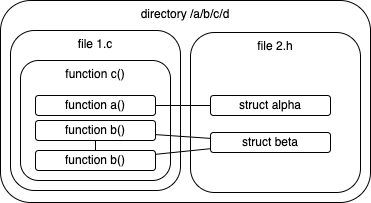
\includegraphics{schema}   

	\item Use a network algorithms - like a hierarchical greedy clustering to achieve superclustering - to automatically identify edges crossing multiple edge boundaries.
	
	\begin{enumerate}
		\item Manually analyze where there are cross-boundary edges between nodes that span directories - those might exist as described in the paper for performance optimizations reasons and such. 
	\end{enumerate}


	\item Use the directory - due to the lack of a namespace concept in C - names of the encompassing structures to derive the bigger building blocks of the architecture.
\end{enumerate}


This approach is overall emphasizing stronger on the 'actual architecture' than the 'desired architecture' - but after more than 2 decades of active work on the Linux kernel, the usage of other resources as comparison material seems to be futile:
Too much research and practical experience has been added to the kernel over time that speaks strongly for the current existing architecture itself being proper and maintainable.


%\makeworkscited %Prints bibliography
	
\end{document}